% Scientific rewrite, October 16, 2026. Results remain development evidence.
\documentclass[letterpaper]{article}
\usepackage[draft]{aaai2027}
\usepackage[hyphens]{url}
\usepackage{graphicx}
\urlstyle{rm}
\def\UrlFont{\rm}
\usepackage{natbib}
\usepackage{caption}
\usepackage{amsmath}
\usepackage{amssymb}
\usepackage{booktabs}
\usepackage{tikz}
\usetikzlibrary{arrows.meta,positioning,calc,fit,backgrounds}
\frenchspacing
\pdfinfo{/TemplateVersion (2027.1)}
\setcounter{secnumdepth}{2}
\newcommand{\best}[1]{\mathbf{#1}}
\newcommand{\todo}[1]{\par\noindent\textbf{Research TODO.} #1\par}
\title{Whole-Tree Learning over Ordered Genealogies\\for Local Ancestry Inference}
\author{Anonymous Authors}
\affiliations{}
\begin{document}
\maketitle

\begin{abstract}
A person's genome contains segments inherited from different ancestral populations. Identifying these segments helps reconstruct population history, but their boundaries can be difficult to recover from genetic data. Inferred genealogies offer a natural representation of shared ancestry: each local tree connects sampled genomes, and the trees change along the chromosome. Learning from this representation requires combining evidence within each tree with continuity across trees. We develop a whole-tree neural model that propagates genetic and reference-panel information through complete genealogies and follows sampled haplotypes along the genome. Structural conditioning marks changes in descendant groups, while recurrent context connects local predictions. On eight European development simulations, the strongest span-accuracy candidate reaches $97.08\pm0.57\%$, compared with $94.45\pm1.15\%$ for the evaluated ARGMix release. Matched controls show that much of the improvement within our model family also follows from continued training. The highest span accuracy and the best boundary score occur in different variants. These findings support whole-tree learning as a promising ancestry framework and identify boundary recovery as a distinct target for model design.
\end{abstract}

\section{Introduction}
Local ancestry inference identifies the ancestral source of each segment of a genome. It can reveal how populations mixed, how ancestry changed through time and how genetic variants moved between populations. In ancient genomics, dated samples provide observations from different stages of this history. A useful predictor must distinguish reference ancestries while respecting both the genealogical relationships between samples and the spatial continuity of ancestry along a chromosome.

An ancestral recombination graph (ARG) represents the changing genealogy of sampled genomes. At any genomic position, a marginal tree connects the sampled haplotypes through common ancestors. Recombination changes this tree along the chromosome. The resulting data have two linked forms of structure: relationships within a tree and correspondence between successive trees. Sampled haplotypes retain their identities, even when their inferred ancestral relationships change.

Recent ancestry methods exploit these genealogical representations. AncestralPaths uses ancestral-path features in the study of ancient Eurasian genomes \citep{eurasians2024}. ARGMix combines genealogical graph representations with genomic sequence modeling \citep{ancientancestry2026}. ARGformer learns representations of genealogical paths \citep{argformer2026}. These approaches motivate a complementary question: how much ancestry information can a compact model recover by processing complete marginal trees and maintaining a continuous sampled-haplotype representation?

A generic sequence of graph embeddings does not directly preserve every sample's relationship to all other samples. Conversely, a set-based graph model does not by itself encode genomic order or physical distance. For genealogies, treating internal-node identifiers as persistent can also introduce a false correspondence. The reliable shared interface is the sampled haplotype. Descendant sets provide an additional structural comparison, but an equal descendant set does not prove that two inferred internal nodes represent the same biological ancestor.

We therefore build a whole-tree model with two complementary computations. Upward and downward messages connect reference and query haplotypes through every node in each local genealogy. A genomic recurrent network then follows each sampled haplotype through the ordered tree sequence. Local changes in descendant groups condition a second tree traversal. We examine whether additional cross-tree context improves this representation using matched episode and memory controls.

The present results support three scientific observations. First, the evaluated whole-tree pipelines exceed the evaluated native ARGMix and AncestralPaths pipelines on the shared European development endpoint. Second, simple local structural features are competitive with the examined cross-tree interactions. Third, span accuracy and tract-boundary recovery favor different variants. This analysis identifies which design choices improve fitted ancestry prediction and which metrics expose remaining errors. The completed comparisons use eight development simulations that have also informed model selection. Independent testing and the remaining native benchmarks are explicit completion items in this working manuscript.

\section{Related Work}
\paragraph{Genealogy-based ancestry inference.}
AncestralPaths accompanies an analysis of the selection landscape and genetic legacy of ancient Eurasians \citep{eurasians2024}. Its ancestral-path formulation distinguishes historical routes that can share the same broad source ancestry. This distinction matters when aligning its output with a four-source classifier. Our comparison uses the released dense classifier and collapses its six path probabilities to four source probabilities. The original study describes a convolutional classifier, whereas the archived executable model is dense. We label the comparison by the executed archive.

ARGMix learns ancestry from genealogical graph representations and genomic context \citep{ancientancestry2026}. We evaluate a current author release with its native model and selection rule, using a disclosed panel adaptation. ARGformer instead learns genealogical path representations with a transformer and supports ancestry assignment by retrieval \citep{argformer2026}. Its American admixture benchmark motivates our separate three-source comparison. A completed ARGformer head-to-head score is not yet available. FLARE uses a haplotype-based local ancestry framework \citep{flare2023} and provides a comparator that does not require the same neural genealogy representation.

These methods differ in what they encode, how they obtain supervision and how they select predictions. A shared observed panel and a common scorer make their ancestry outputs comparable on that endpoint. They do not make the comparison a controlled test of architecture alone.

\paragraph{Learning from collections of graphs.}
Graph Set Transformer interleaves node-level propagation and set-wide contextual modeling rather than first reducing each graph to a fixed embedding \citep{gst2026}. This provides a relevant motivation for exchanging information before final graph readout. Our setting adds genomic order, unequal interval lengths and persistent sampled entities. These properties determine which cross-tree correspondences have a biological interpretation.

Temporal graph state-space models study recurrent state on changing graphs \citep{graphssm2024}. Gated recurrent units provide an established sequence mechanism \citep{gru2014}. Our graph sweeps, gated recurrence, pooling and residual conditioning use established ingredients. The empirical question is whether their genealogical organization improves ancestry inference, and whether a proposed cross-tree interaction adds value beyond matched local and continued-training controls.

\section{Whole-Tree Ancestry Model}
\subsection{Inputs and Prediction Target}
Let $T_t=(V_t,E_t)$ be the inferred marginal tree on interval $I_t$ of length $w_t$. The same sampled haplotypes appear in every tree. Let $v_t(q)$ denote the node of sampled haplotype $q$ in tree $t$. Inferred internal nodes need not correspond across trees.

The observed inputs are phased genetic variants, inferred topology and branch ages, sample ages, and source labels for the reference panel. The source labels of query haplotypes are masked. The model predicts a probability vector $p_{tq}$ over Anatolian farmer (Ana), Caucasus hunter-gatherer (CHG), western hunter-gatherer (WHG) and eastern hunter-gatherer (EHG) ancestry. Training uses simulated ancestry labels as external supervision. These labels do not define input features, inferred trees or genomic intervals.

Figure~\ref{fig:architecture} shows the data representation and the strongest span-accuracy variant. The central design preserves the complete genealogy during graph propagation and the complete sequence of marginal-tree contexts during genomic recurrence.

\begin{figure*}[t]
\centering
% Original editable vector figure. Illustrative genealogies, not experimental data.
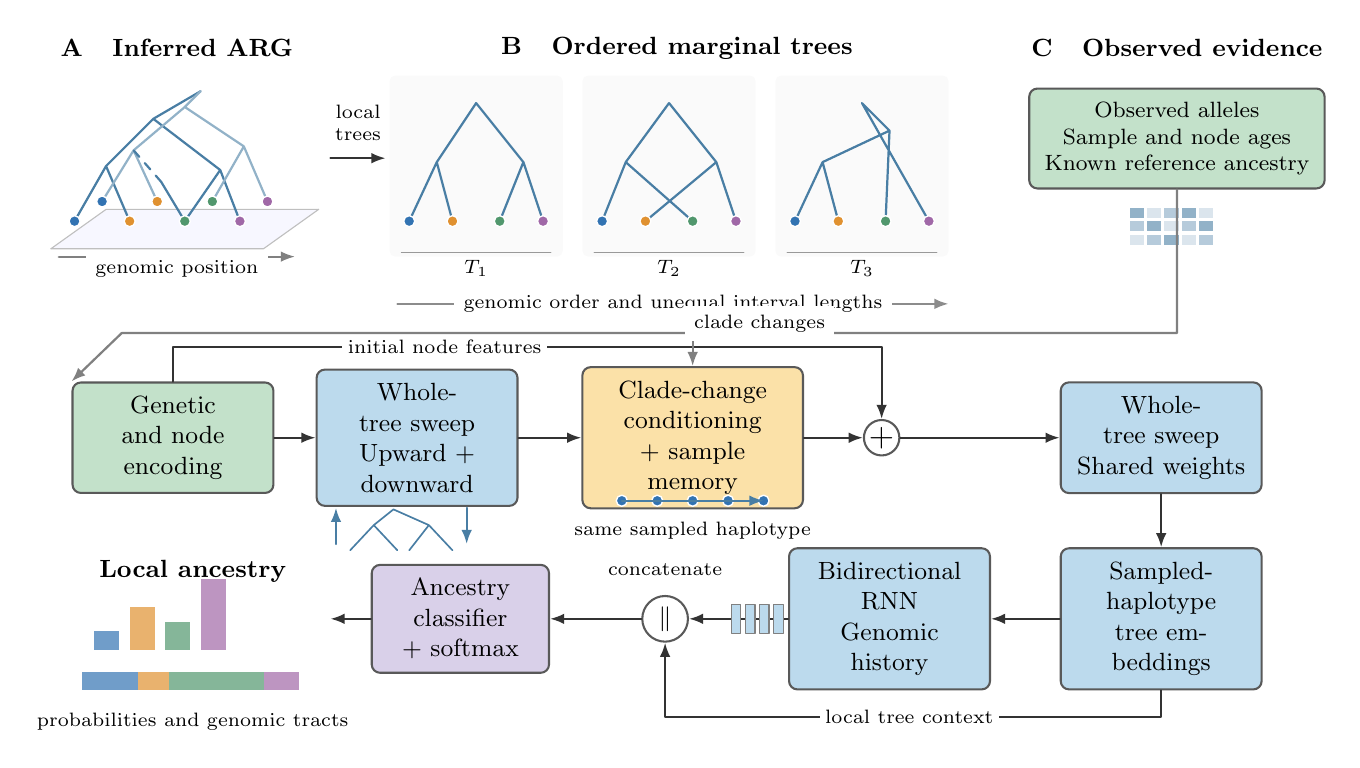
\begin{tikzpicture}[
 x=1cm,y=1cm,>=Latex,
 line cap=round,line join=round,
 flow/.style={-{Latex[length=1.8mm]},line width=.8pt,draw=black!80},
 aux/.style={flow,draw=black!50},
 box/.style={draw=black!65,rounded corners=3pt,line width=.75pt,align=center,
 minimum height=.92cm,text width=2.2cm,inner sep=5pt,font=\small},
 leaf/.style={circle,draw=white,line width=.5pt,minimum size=4pt,inner sep=0pt},
 vec/.style={draw=black!50,line width=.45pt,minimum width=.12cm,minimum height=.37cm,inner sep=0pt},
 lab/.style={font=\small,align=center}
]
\definecolor{treeblue}{RGB}{73,126,164}
\definecolor{genegreen}{RGB}{195,225,202}
\definecolor{localgold}{RGB}{251,225,168}
\definecolor{seqblue}{RGB}{188,218,237}
\definecolor{outpurple}{RGB}{217,208,233}
\definecolor{samplea}{RGB}{50,115,178}
\definecolor{sampleb}{RGB}{224,145,48}
\definecolor{samplec}{RGB}{81,151,109}
\definecolor{sampled}{RGB}{160,104,167}
% Upper row: data and correspondence.
\node[lab,font=\small\bfseries] at (1.7,9.7) {A\quad Inferred ARG};
\fill[blue!3] (.1,7.15)--(2.8,7.15)--(3.5,7.65)--(.8,7.65)--cycle;
\draw[black!25] (.1,7.15)--(2.8,7.15)--(3.5,7.65);
\draw[black!25] (.1,7.15)--(.8,7.65)--(3.5,7.65);
\draw[flow,black!50] (.2,7.05)--(3.2,7.05);
\node[font=\scriptsize,fill=white] at (1.7,6.9) {genomic position};
\draw[treeblue,thick]
 (.4,7.5)--(.8,8.2)--(1.4,8.8)--(2.0,9.15)
 (1.1,7.5)--(.8,8.2)
 (1.8,7.5)--(2.25,8.15)--(1.4,8.8)
 (2.5,7.5)--(2.25,8.15);
\draw[treeblue!60,thick]
 (.75,7.75)--(1.15,8.4)--(1.8,8.95)--(2.0,9.15)
 (1.45,7.75)--(1.15,8.4)
 (2.15,7.75)--(2.55,8.45)--(1.8,8.95)
 (2.85,7.75)--(2.55,8.45);
\draw[treeblue,thick,dashed] (1.5,8.0)--(1.15,8.4);
\draw[treeblue,thick] (1.5,8.0)--(1.8,7.5);
\foreach \x/\c in {.4/samplea,1.1/sampleb,1.8/samplec,2.5/sampled}
 \node[leaf,fill=\c] at (\x,7.5) {};
\foreach \x/\c in {.75/samplea,1.45/sampleb,2.15/samplec,2.85/sampled}
 \node[leaf,fill=\c] at (\x,7.75) {};
\draw[flow] (3.65,8.3)--(4.35,8.3);
\node[font=\scriptsize,align=center] at (4.0,8.75) {local\\trees};
\node[lab,font=\small\bfseries] at (8.05,9.7) {B\quad Ordered marginal trees};
\foreach \offset/\name in {4.55/1,7.0/2,9.45/3}{
 \begin{scope}[shift={(\offset,0)}]
 \fill[black!2,rounded corners=2pt] (-.15,7.05) rectangle (2.05,9.35);
 \draw[black!40] (0,7.1)--(1.9,7.1);
 \node[font=\scriptsize] at (.95,6.9) {$T_{\name}$};
 \end{scope}
}
% Tree 1 pairs ab and cd.
\draw[treeblue,thick] (4.65,7.5)--(5.0,8.25)--(5.5,9.0)
 (5.2,7.5)--(5.0,8.25)
 (5.8,7.5)--(6.1,8.25)--(5.5,9.0)
 (6.35,7.5)--(6.1,8.25);
% Tree2 pairs ac and bd, leaf order persistent.
\draw[treeblue,thick] (7.10,7.5)--(7.4,8.25)--(7.95,9.0)
 (8.25,7.5)--(7.4,8.25)
 (7.65,7.5)--(8.55,8.25)--(7.95,9.0)
 (8.80,7.5)--(8.55,8.25);
% Tree3 changes a clade.
\draw[treeblue,thick] (9.55,7.5)--(9.9,8.25)--(10.75,8.65)--(10.4,9.0)
 (10.10,7.5)--(9.9,8.25)
 (10.7,7.5)--(10.75,8.65)
 (11.25,7.5)--(10.4,9.0);
\foreach \offset in {4.55,7.0,9.45}{
 \foreach \dx/\c in {.1/samplea,.65/sampleb,1.25/samplec,1.8/sampled}
  \node[leaf,fill=\c] at (\offset+\dx,7.5) {};
}
\draw[flow,black!45] (4.5,6.45)--(11.5,6.45);
\node[font=\scriptsize,fill=white] at (8,6.45) {genomic order and unequal interval lengths};
\node[lab,font=\small\bfseries] at (14.4,9.7) {C\quad Observed evidence};
\node[box,fill=genegreen,text width=3.4cm,font=\footnotesize] (evidence) at (14.4,8.55)
 {Observed alleles\\Sample and node ages\\\mbox{Known reference ancestry}};
% Tiny allele matrix, with no software notation.
\foreach \row in {0,1,2}{
 \foreach \col in {0,1,2,3,4}{
  \pgfmathtruncatemacro{\shade}{mod(\row+\col,3)*20+20}
  \fill[treeblue!\shade] (13.8+.22*\col,7.2+.17*\row)
    rectangle ++(.18,.13);
 }
}
% Middle flow with explicit residual sum and base skip.
\node[box,fill=genegreen] (encode) at (1.65,4.75) {Genetic and node\\encoding};
\node[box,fill=seqblue] (first) at (4.75,4.75) {Whole-tree sweep\\Upward + downward};
\node[box,fill=localgold,text width=2.45cm,minimum height=1.25cm] (resid) at (8.25,4.75)
 {Clade-change\\conditioning\\+ sample memory};
\node[circle,draw=black!65,fill=white,line width=.75pt,minimum size=.45cm,
 inner sep=0pt,font=\large] (plus) at (10.65,4.75) {$+$};
\node[box,fill=seqblue] (second) at (14.2,4.75) {Whole-tree sweep\\Shared weights};
\draw[flow] (encode)--(first);
\draw[flow] (first)--(resid);
\draw[flow] (resid)--(plus);
\draw[flow] (plus)--(second);
\draw[flow] (encode.north)--(1.65,5.9)--(10.65,5.9)--(plus.north);
\node[font=\scriptsize,fill=white,inner sep=2pt] at (5.1,5.9) {initial node features};
\draw[aux] (evidence.south)--(14.4,6.08)--(1.0,6.08)--(encode.north west);
\draw[aux] (8.25,6.2)--(resid.north);
\node[font=\scriptsize,align=center,fill=white] at (9.1,6.2) {clade changes};
% Whole-tree mini glyph and memory glyph.
\draw[treeblue,line width=.6pt] (3.9,3.32)--(4.2,3.64)--(4.5,3.32)
 (4.2,3.64)--(4.45,3.84)--(4.9,3.64)
 (4.9,3.64)--(4.65,3.32) (4.9,3.64)--(5.2,3.32);
\draw[flow,treeblue] (3.72,3.40)--(3.72,3.86);
\draw[flow,treeblue] (5.38,3.86)--(5.38,3.40);
\foreach \x/\c in {7.35/samplea,7.8/samplea,8.25/samplea,8.7/samplea,9.15/samplea}{
 \node[leaf,fill=\c] at (\x,3.95) {};
}
\draw[flow,treeblue,line width=.6pt] (7.35,3.95)--(9.15,3.95);
\node[font=\scriptsize] at (8.25,3.57) {same sampled haplotype};
% Lower row, right to left with local skip.
\node[box,fill=seqblue] (sample) at (14.2,2.45) {Sampled-haplotype\\tree embeddings};
\node[box,fill=seqblue] (rnn) at (10.75,2.45)
 {Bidirectional RNN\\Genomic history};
\node[circle,draw=black!65,fill=white,line width=.75pt,minimum size=.58cm,
 inner sep=0pt,font=\small] (concat) at (7.9,2.45) {$\Vert$};
\node[box,fill=outpurple,text width=1.9cm] (head) at (5.3,2.45) {Ancestry classifier\\+ softmax};
\draw[flow] (second)--(sample);
\draw[flow] (sample)--(rnn);
\draw[flow] (rnn)--(concat);
\draw[flow] (concat)--(head);
\draw[flow] (sample.south)--(14.2,1.2)--(7.9,1.2)--(concat.south);
\node[font=\scriptsize,fill=white,inner sep=2pt] at (11,1.2) {local tree context};
% vectors at concat show operation visually.
\foreach \x/\c in {8.8/seqblue,8.98/seqblue,9.16/seqblue,9.34/seqblue}
 \node[vec,fill=\c] at (\x,2.45) {};
\node[font=\scriptsize] at (7.9,3.08) {concatenate};
% Output probabilities and tracks.
\draw[flow] (head.west)--(3.65,2.45);
\node[lab,font=\small\bfseries] at (1.9,3.05) {Local ancestry};
\foreach \x/\height/\c in {.65/.25/samplea,1.1/.55/sampleb,1.55/.36/samplec,2.0/.9/sampled}{
 \fill[\c!70] (\x,2.05) rectangle ++(.32,\height);
}
\foreach \x/\wid/\c in {.5/.7/samplea,1.2/.4/sampleb,1.6/1.2/samplec,2.8/.45/sampled}
 \fill[\c!70] (\x,1.55) rectangle ++(\wid,.22);
\node[font=\scriptsize] at (1.9,1.14) {probabilities and genomic tracts};
\end{tikzpicture}

\caption{Whole-tree ancestry inference. \textbf{A:} An inferred ARG describes genealogical change along the genome. \textbf{B:} Its ordered marginal trees retain the same sampled haplotypes, shown by repeated colors. Internal ancestors can change. \textbf{C:} Observed alleles, sample ages and reference labels supply features. Two shared whole-tree sweeps propagate information upward and downward. Structural residuals mark clade changes and provide local conditioning. In the stable-leaf variant, cut-level context is carried along persistent sampled haplotypes and added before the second sweep. A bidirectional recurrent network follows each sampled haplotype through the genomic sequence. Its history is concatenated with local tree context to predict ancestry probabilities and tracts. The drawing is schematic, with four sampled haplotypes for clarity.}
\label{fig:architecture}
\end{figure*}

\subsection{Genetic Evidence and Whole-Tree Propagation}
The genetic encoder summarizes each haplotype's called alleles relative to observed donor and panel allele frequencies. Mean and maximum pooling within a tree interval produce a local genetic representation. This representation is combined with sample age and the known reference label, where available. Inferred node ages and node roles provide features for internal ancestors. These quantities produce an initial node state $b_v$. Branch geometry and mutation-concordance summaries determine message gates.

The first traversal propagates information from sampled leaves toward the root. For parent $v$ and child $u$,
\begin{align}
m_{u\to v}
 &=\frac{g_u^\uparrow\odot W_\uparrow h_u}{\max(1,d_v)},\\
s_v&=\sum_{u\in\operatorname{child}(v)}m_{u\to v},\\
h_v&=\operatorname{LN}\!\left(
 b_v+\tanh(A_\uparrow[b_v,s_v]+a_\uparrow)\right),
\end{align}
where $d_v$ is the number of children, $g_u^\uparrow$ is an observed-feature gate and brackets denote concatenation.

The downward traversal supplies the context outside each child's branch. Its parent context excludes the recipient's own upward message,
\begin{equation}
c_{v\setminus u}=o_v+b_v+s_v-m_{u\to v}.
\label{eq:cavity}
\end{equation}
A gated learned transformation maps this context to the child's outside state $o_u$. Root outside states are zero. Excluding the recipient contribution prevents its immediate return as outside evidence. A learned projection of the sampled node's upward and outside states gives its local tree representation. Both traversals visit every native node.

\subsection{Structural Conditioning}
For a node $v$, let $C_t(v)$ be the set of its descendant sampled haplotypes. We compare proper clades between adjacent trees. A proper clade contains at least two sampled haplotypes and excludes the full panel. Equal clades along a unary chain use the deepest structural representative.

A node receives a gained flag $g_v$ when its clade is absent from the preceding tree and a lost flag $\ell_v$ when it is absent from the following tree. End-of-sequence missing-neighbor flags are zero. These flags describe observed topology changes rather than ancestral identity. They condition a local residual,
\begin{equation}
\Delta_v^{\mathrm{clade}}=
O\!\left[
g_v(Uh_v\odot Vh_v)
-\ell_v(Uh_v\odot Wh_v)
\right].
\label{eq:clade}
\end{equation}
The projections use a low-rank intermediate representation. A second whole-tree sweep receives $b_v+\Delta_v$ and reuses the first sweep's learned weights and observed gates.

We also examine contiguous episodes of the same proper clade. For episode member $i$, a span-weighted context excludes its own tree,
\begin{equation}
\bar h_{-i}=
\frac{\sum_{j\in E(i)}w_jh_j-w_ih_i}
     {\sum_{j\in E(i)}w_j-w_i}.
\label{eq:episode}
\end{equation}
Episodes with at least two members receive the residual
\begin{equation}
\Delta_i^{\mathrm{episode}}
 =O_e\!\left[(U_eh_i)\odot(V_e\bar h_{-i})+W_eh_i\right].
\end{equation}
The matched local control substitutes $h_i$ for $\bar h_{-i}$ on the same eligible nodes. It retains the same parameter count, initialization and training budget. This control asks whether foreign-tree states help beyond the additional local transformation.

\subsection{Memory along Persistent Samples}
The strongest span-accuracy candidate adds stable-leaf memory to the local-control model. A time cut at 350 generations groups sampled haplotypes by their observed ancestor at that cut. A sample older than the cut retains its sampled node. This cut is computed from inferred node ages, without ancestry labels.

For cut group $k$ in tree $t$, a learned projection of upward and outside context gives a forcing vector $f_{tk}$. Let $k_t(q)$ denote haplotype $q$'s group. A forward memory follows the same sampled haplotype across trees,
\begin{equation}
z^\rightarrow_{tq}
=\rho_t z^\rightarrow_{t-1,q}
 +(1-\rho_t)f_{t,k_t(q)},
\qquad
\rho_t=\exp(-w_t/\lambda).
\label{eq:memory}
\end{equation}
The first state is initialized by its forcing. A reverse scan uses the corresponding reverse order. The positive learned distance scale $\lambda$ lets physical span determine the amount of retained history.

The two directions are averaged, pooled over the current cut group, and centered by subtracting the current forcing. A learned output projection injects this residual at that group's representative before the second tree sweep. This mechanism preserves sample identity even when cut groups change. The shared framework also permits pair-cell memory, which transports history through intersections of adjacent cut groups, and an adjacent-marginal control that discards the additional intersection conditioning. We compare these rules with continued training without added memory.

\subsection{Genomic Context and Ancestry Readout}
The second tree sweep produces a local representation $e_{tq}$ for every sampled haplotype. A bidirectional recurrent network receives this representation together with interval length and neighboring interval distances,
\begin{equation}
r_{1:T,q}=\operatorname{BiGRU}
 \bigl([e_{tq},\operatorname{geometry}(I_t)]_{t=1}^T\bigr).
\end{equation}
The classifier uses both local and genomic information,
\begin{equation}
p_{tq}=\operatorname{softmax}
 \left(\operatorname{MLP}([e_{tq},r_{tq}])\right).
\end{equation}
The recurrent computation retains all tree intervals and all sampled haplotypes. Query selection occurs only at readout. Predictions are constant within each native tree interval, which limits the possible positions of ancestry transitions.

\section{Experimental Design}
\subsection{European Ancestry Panel}
The shared European development panel contains 476 diploid individuals, comprising 952 phased haplotypes. Of these, 266 are reference haplotypes and 686 are queries. The query cohorts include present-day individuals, Bronze Age individuals, Bronze Age Anatolians (BAA), Neolithic farmers (Neo) and Yamnaya (Yam). The released cohort names are retained. Bronze Age is an approximate correspondence to the preprint's Post-Neolithic category, rather than a verified identical panel.

We generated 32 training and eight development-validation simulations, each spanning 2\,Mb, from the released ancient-European demographic formulation. Relate inferred the genealogies from observed variants \citep{relate2019}. The simulation and inference parameters are given in the supplement, including demographic admixture events and sample-panel sizes. Simulation identity determines the split before any rows, tree intervals or sequence chunks are constructed.

The four-source endpoint uses Ana, CHG, WHG and EHG. AncestralPaths' six path probabilities are collapsed before class assignment,
\begin{equation}
(p_{\mathrm{Ana}},p_{\mathrm{CHG}},p_{\mathrm{WHG}},p_{\mathrm{EHG}})
=(p_1+p_5,p_2+p_6,p_3,p_4).
\end{equation}
The native six-path task is distinct from this derived four-source endpoint.

\subsection{Metrics and Statistical Unit}
All European pipelines are scored on the same fixed 100\,bp bins, clipped to inferred coverage. Ancestry truth is intersected with these bins to obtain the true physical mass $m_{iqc}$ of source $c$ for query $q$ in bin $i$. Span accuracy is
\begin{equation}
A=\frac{\sum_{iqc}m_{iqc}
  \mathbf{1}\{c=\arg\max_k p_{iqk}\}}
 {\sum_{iqc}m_{iqc}}.
\end{equation}
The primary endpoint gives each simulation equal weight and considers the 182 present-day query haplotypes. Cohort and all-query results are secondary. Negative log-likelihood (NLL) weights true-class log probabilities by the same physical mass.

Span accuracy emphasizes genomic extent. Boundary precision, recall and F1 instead evaluate transitions using one-to-one positional matching within 1\,kb. This matcher ignores source-transition identity. We report mean and sample SD across the eight simulations. These SDs quantify variation among simulations for one fitted model per condition, rather than variability across training seeds or a confidence interval.

\subsection{Native Comparators and Matched Controls}
AncestralPaths retains the released dense classifier, six outputs and five-epoch fit. Its bounded sampler has a shortfall in BAA path-six rows, as detailed in the supplement. ARGMix retains the current author's released model, its 15-reference representation without ancestor nodes, genomic sequence modeling and native early stopping. A full-panel slot and metadata adaptation lets it process the common observed roster. The preprint instead specifies 25 references and three ancestor nodes, and the public release does not support ancestor inputs. We label the evaluated release condition explicitly. The model's inner selection rule remains unchanged.

Our model also receives observed SNP features. The native pipelines differ in representations, row sampling, supervision units, training exposure and checkpoint selection. The common endpoint therefore compares fitted ancestry pipelines. It does not assign their entire difference to the neural architecture.

Within our model family, matched controls isolate narrower questions. Clade-event tensor and event-MLP models share added capacity and training. Local flags use the same added parameter count and continuation budget. Episode models differ only in foreign versus own-state conditioning. The final four-arm memory comparison starts from the same local-control checkpoint and gives every arm the same additional training budget. All model weights remain trainable. Training details and cumulative exposure are in the supplement.

\todo{Complete the untouched European assessment and common-data native ARGformer comparison. For a comparison with the ARGMix preprint's numerical tables, verify the original sample roster, reference eligibility, genomic map, observation pipeline and scoring protocol. The available author release postdates the preprint and does not support its ancestor inputs. Recover the original paper-era model, training specification and checkpoint. A 25-reference release sensitivity would still have zero ancestors and must be named separately. The completed 476-diploid condition remains a shared development comparison.}

\section{Results}
\subsection{Shared European Development Performance}
Table~\ref{tab:pipeline} summarizes the evaluated pipelines. Stable-leaf memory reaches $97.0778\pm0.5674\%$ present-day span accuracy, compared with $94.4461\pm1.1491\%$ for current native ARGMix and $93.7830\pm0.8385\%$ for the derived AncestralPaths output. The stable-leaf--ARGMix difference is 2.63 percentage points for these fitted pipelines.

\begin{table}[t]
\centering
\small
\begin{tabular}{@{}lr@{}}
\toprule
Pipeline & Span accuracy (\%) $\uparrow$\\
\midrule
Released AncestralPaths, derived C4 & $93.78\pm0.84$\\
Current native ARGMix & $94.45\pm1.15$\\
Whole-tree base & $95.49\pm0.83$\\
Local clade flags & $96.58\pm0.60$\\
Episode local control & $96.82\pm0.61$\\
Foreign-episode context & $96.83\pm0.59$\\
Continued-training control & $97.00\pm0.50$\\
Stable-leaf memory & $\best{97.08\pm0.57}$\\
\bottomrule
\end{tabular}
\caption{Shared European development endpoint on 182 present-day query haplotypes. Values are mean$\pm$simulation SD across eight 2\,Mb simulations. The best observed mean is bold. Inputs, training exposure and model selection differ between pipeline families. This is not a reproduction of published table values.}
\label{tab:pipeline}
\end{table}

The progression within the neural family also increases training exposure. The continued-training control reaches $97.00\%$ without adding memory. Stable leaves exceed that control by only $0.0778$ points, and the paired episode comparison adds only $0.0096$ points for foreign states. Thus the larger pipeline gain does not establish that cross-tree message exchange is its cause.

The source cohorts have different prediction difficulty (Table~\ref{tab:cohorts}). The local-flag model exceeds the native comparators in every listed cohort under this condition. Scores are highest for the ancient aggregate. This does not demonstrate equal performance on empirical ancient DNA, since source mixtures, sampling ages and tract structures differ between cohorts.

\begin{table*}[t]
\centering
\small
\begin{tabular}{@{}lrrrrr@{}}
\toprule
Cohort & Query haplotypes & AncestralPaths, C4 & ARGMix & Whole-tree base & Local flags\\
\midrule
Present-day &182&$93.78\pm0.84$&$94.45\pm1.15$&$95.49\pm0.83$&$\best{96.58\pm0.60}$\\
Bronze Age &162&$94.76\pm1.18$&$97.71\pm0.75$&$98.17\pm0.80$&$\best{99.07\pm0.32}$\\
BAA &14&$96.94\pm1.32$&$98.44\pm1.02$&$98.90\pm0.89$&$\best{99.02\pm1.07}$\\
Neo &302&$97.57\pm0.27$&$99.30\pm0.26$&$99.41\pm0.13$&$\best{99.53\pm0.18}$\\
Yam &26&$95.43\pm1.41$&$99.22\pm0.90$&$98.96\pm1.31$&$\best{99.86\pm0.19}$\\
Ancient &504&$96.54\pm0.32$&$98.76\pm0.31$&$98.98\pm0.32$&$\best{99.39\pm0.16}$\\
All queries &686&$95.81\pm0.45$&$97.61\pm0.50$&$98.05\pm0.43$&$\best{98.64\pm0.26}$\\
\bottomrule
\end{tabular}
\caption{Cohort span accuracy (\%), mean$\pm$simulation SD. Bold identifies the best mean within each row. Ancient and all-query rows aggregate the cohorts above them. This completed cohort comparison concerns the local-flag model, rather than the later stable-leaf model. Bronze Age has not been established as identical to the published Post-Neolithic panel.}
\label{tab:cohorts}
\end{table*}

\subsection{What Does Cross-Tree Context Add?}
Local clade flags outperform the examined clade-event tensor interaction by $0.3104\pm0.2588$ accuracy points and the matched event MLP by $0.3771\pm0.2165$ points. The simpler structural control therefore captures useful information that these interactions need not exchange explicitly. In a later matched comparison, foreign-episode context exceeds own-state conditioning by $0.0096\pm0.1527$ points. This falls below the registered practical-gain threshold of 0.10 points.

The ordered-memory comparison tests whether a richer transport rule improves over stable samples and continued training (Table~\ref{tab:memory}). Pair-cell memory exceeds its adjacent-marginal control by $0.0137\pm0.0243$ accuracy points. It is below stable-leaf memory by $0.0138\pm0.0384$ points. Neither registered utility criterion is met: a gain of at least 0.10 accuracy points without a boundary-F1 decrease, or a gain of at least 1.00 boundary-F1 point with no more than 0.05 accuracy points lost, against every control. These thresholds are practical development criteria.

\begin{table}[t]
\centering
\small
\begin{tabular}{@{}lrr@{}}
\toprule
Memory condition & Accuracy $\uparrow$ & Boundary F1 $\uparrow$\\
\midrule
Pair-cell & $97.064\pm0.560$ & $18.93\pm1.42$\\
Adjacent marginal & $97.050\pm0.580$ & $18.85\pm1.05$\\
Stable leaves & $\best{97.078\pm0.567}$ & $18.38\pm1.31$\\
Continued training & $97.000\pm0.498$ & $\best{19.05\pm1.43}$\\
\bottomrule
\end{tabular}
\caption{Matched ordered-memory comparison, mean$\pm$simulation SD in percent. All arms finish the same additional training budget. Checkpoint selection is individual to each arm. Bold identifies the largest mean in each metric. Boundary tolerance is 1\,kb.}
\label{tab:memory}
\end{table}

Stable leaves have the highest span accuracy, while continued training has the highest boundary F1. Their paired differences are $+0.0778$ accuracy points and $-0.6682$ boundary-F1 points. This tradeoff is central to evaluating a method intended to recover ancestry tracts.

\subsection{Tract Boundaries Remain Difficult}
Table~\ref{tab:boundaries} shows that improvements in span accuracy can accompany better boundary F1 relative to native pipelines, while still leaving most true transitions unrecovered. Local flags reach $18.05\pm1.84\%$ F1. AncestralPaths has the highest recall in this comparison, at a much lower precision.

\begin{table}[t]
\centering
\small
\begin{tabular}{@{}lrrr@{}}
\toprule
Pipeline & Prec. $\uparrow$ & Recall $\uparrow$ & F1 $\uparrow$\\
\midrule
AP (C4)&$3.95\pm0.48$&$\best{32.36\pm2.06}$&$7.03\pm0.78$\\
ARGMix&$9.16\pm1.49$&$16.41\pm2.22$&$11.74\pm1.73$\\
Tree base&$10.71\pm1.21$&$17.99\pm2.01$&$13.42\pm1.47$\\
Local flags&$\best{15.21\pm2.01}$&$22.30\pm1.86$&$\best{18.05\pm1.84}$\\
\bottomrule
\end{tabular}
\caption{Present-day boundary metrics (\%), with AP denoting AncestralPaths. Values are mean$\pm$simulation SD at 1\,kb tolerance. The best mean in each column is bold, including the native comparator's recall. Matching is positional and does not require the correct source-transition identity.}
\label{tab:boundaries}
\end{table}

A diagnostic of frozen whole-tree-base predictions separates representation from recognition. Of 4,008 true changes, 1,094 have no native interval edge within 1\,kb. Yet 2,195 of the model's 3,289 missed changes do have a nearby candidate. Finer readout alone would therefore address only part of the problem. Short false ancestry islands also contribute disproportionately to extra boundaries: islands of at most 10\,kb account for $35.46\pm2.71\%$ of extra boundaries but only $3.83\pm0.73\%$ of erroneous physical mass. This explains why a span-based ranking can understate fragmentation.

\subsection{American Admixture Benchmark}
A separate 30\,Mb American simulation contains 600 reference and 1,000 query haplotypes with EUR, EAS and AFR source classes. Released FLARE calls reach $98.0100\%$ accuracy and $97.7151\%$ macro F1 on 10,000 predetermined focal records. This is one validation simulation, so no between-simulation SD is available. The endpoint counts focal records rather than physical span.

\todo{Complete our model and native ARGformer on the same American observations, reference/query identities and focal support. Add multi-simulation uncertainty and verify the published demographic and prediction settings before comparing with its Table~1. The current FLARE score alone establishes no head-to-head ranking.}

\subsection{Application to Ancient Danish Genomes}
We applied a frozen foreign-episode model to ten ancient Danish query individuals and eight proxy-reference individuals from the imputed genomes analyzed by \citet{eurasians2024}. Five earlier individuals date to 5.44--5.67\,ka cal BP and five later individuals to 3.97--4.26\,ka cal BP. Three fixed 10\,Mb windows on chromosomes 20--22 contain 1,158 inferred trees and 8,587 qualified site records.

The model received original phased genotypes and was not fitted again. Person-weighted, span-integrated assignments are 14.27 percentage points higher for EHG and 5.52 points higher for CHG in the later group. The EHG contrast is positive on each chromosome. The pooled CHG contrast depends on chromosome 21, and becomes $-0.68$ points when that chromosome is omitted. Independent genotype-affinity contrasts using the shared imputation resource do not support the registered directions. These model assignments are descriptive outputs, without local ancestry truth or calibrated mixture fractions. The application illustrates behavior on empirical genealogies rather than confirming a population-history hypothesis.

\section{Discussion}
Whole-tree learning provides a direct way to combine reference ancestry, genetic variation and genealogical structure. Its sampled-haplotype interface preserves correspondence along the genome without assuming persistent inferred ancestors. The shared European development comparison is encouraging for this representation. Its biological value must nevertheless be judged by both the amount of correctly assigned sequence and the placement of transitions.

The matched controls constrain the architectural interpretation. Local structural conditioning is competitive with the examined event interactions, foreign-episode context provides little added accuracy over local conditioning, and richer pair-cell memory does not outperform the simpler controls under the registered criteria. Continued training explains much of the later improvement. The present evidence supports this ancestry framework and its comparative analysis, while the contribution of a distinct cross-tree operator remains an open research question.

The external evaluations also have specific scope. Development validation has been reused, native models retain different training and input choices, and the completed panel is not a verified recreation of the published tables. The Danish application has no ancestry ground truth. A separate trade-network diagnostic finds persistence stronger than the tested learned memory models (Supplement), so that experiment does not support a broad generality claim. Independent ancestry tests and completed native benchmarks are the next basis for a stronger conclusion.

\section{Conclusion}
We study local ancestry through complete inferred genealogies linked by persistent sampled haplotypes. Whole-tree propagation, structural conditioning and genomic recurrence achieve promising development span accuracy. Matched controls show that additional cross-tree memory yields small gains and can reduce boundary quality. These results motivate ancestry models that recover tract structure as well as genomic mass, with final claims tied to independent tests and faithful native comparisons.

\paragraph{Code availability.}
Source code, experiment configurations and full results are available at \url{https://github.com/alexeyshmelev/ARG-GNN}.

\bibliography{references}

\clearpage
\appendix
\section*{Supplementary Material}
\suppressfloats[t]
\section{Simulation Design and Biological Parameters}
\label{app:simulation}
The European condition follows the released AncestralPaths formulation associated with \citet{eurasians2024}. Table~\ref{tab:demography} gives its backward-time events. The census at 350 generations defines ancestry supervision before the older source-population mergers. It is separate from the model's observed tree cut.

The panel contains 91 diploids sampled at age zero, together with the released ancient age roster: 81 Bronze Age, seven BAA, 151 Neo and 13 Yam diploids. Pure-reference diploids comprise 51 WHG, 43 EHG, 25 Ana and 14 CHG. This totals 343 query and 133 reference diploids.

Simulations use the Hudson coalescent, discrete genomic coordinates, a uniform recombination rate of $10^{-8}$ per base per generation and JC69 mutations at $1.25\times10^{-8}$ per base per generation \citep{msprime2022}. The released formulation supplies the demographic events and ancient roster. The 2\,Mb sequence length and simulation split define our development condition.

\begin{table}[htbp]
\centering
\small
\begin{tabular}{@{}rll@{}}
\toprule
Time (gen.) & Descendant & Ancestral sources\\
\midrule
166 & Present/Bronze & $0.5$ Neo, $0.5$ Yam\\
169 & BAA & $0.25$ CHG, $0.75$ Ana\\
177 & Yam & $0.5$ CHG, $0.5$ EHG\\
259 & Neo & $0.25$ WHG, $0.75$ Ana\\
600 & WHG, EHG & Shared NE ancestor\\
800 & CHG, Ana & Shared WA ancestor\\
1,500 & NE, WA & Common trunk\\
\bottomrule
\end{tabular}
\caption{Executed European demographic events, following the released formulation associated with AncestralPaths. Mixture coefficients are backward-time ancestral proportions. This is a simulation-design table, so no performance winner is applicable.}
\label{tab:demography}
\end{table}

Population sizes are 50,000 for Present/Bronze and Neo, 20,000 for Yam and BAA, 3,000 for EHG and CHG, 2,000 for WHG, and 5,000 for Ana. The older NE, WA and trunk populations each have size 15,000. Growth and between-event migration rates are zero. The original ancient sampling dates are retained in generations.

Relate uses the observed biallelic variant panel and sample ages. Its initial effective haploid size is 30,000, its mutation rate is $1.25\times10^{-8}$, and years are converted using 28 years per generation. The European condition includes five population-size estimation iterations and final branch-length re-estimation. All applicable European model adapters consume the same post-estimation tree reconstruction. Mutation-concordance features are computed from observed alleles on these inferred trees.

\todo{Before describing any benchmark as a published-paper reproduction, resolve the original ARGMix panel and map configuration and the correspondence between its Post-Neolithic samples and the executed Bronze Age roster. For the American comparison, finalize a source-cited demographic table and focal-sampling protocol alongside the native results.}

\section{Training and Model Hyperparameters}
\label{app:training}
The genetic site encoder has two hidden layers of width 32. It receives donor log-frequency features for the called allele, corresponding availability indicators, the panel frequency of that allele, site entropy and a call indicator. The eight donor groups combine the four reference ancestries with sample ages below or at least 350 generations. Allele-frequency estimates use additive pseudocount 0.5. If any source class represented in a reference age group has no called alleles at a site, all represented classes in that age group are masked for that site. Mean and maximum pooling are combined with call count, missing-pool status and interval span. Leaf features also include the known four-source reference annotation, unknown-label status and sample age. Internal-node features include inferred age, root status and sampled-node status.

Tree hidden states have width 32, residual projections have rank eight, and the bidirectional genomic recurrent network has width 32 per direction. The classifier combines a 32-dimensional local representation and 64-dimensional recurrent history, then maps through width 32 to four ancestry scores. Memory adds 513 parameters and initializes its length scale to 5\,kb, constrained to 100\,bp--100\,kb. Residual output projections start at zero.

The loss is physical-span cross-entropy over all 686 query haplotypes,
\begin{equation}
\mathcal L=-\frac{\sum_{tqc} M_{tqc}\log p_{tqc}}
                  {\sum_{tqc} M_{tqc}},
\qquad
M_{tqc}=\sum_{i:r(i)=t}m_{iqc}.
\end{equation}
Here $r(i)$ maps an original scored bin to its native tree interval. Since predictions are constant within an interval, summing its target masses preserves the original objective. A whole simulated chromosome is one optimization example.

Each development stage completes 30 passes over 32 training simulations, or 960 optimizer updates. AdamW uses learning rate $10^{-3}$, weight decay $10^{-4}$, betas $(0.9,0.999)$ and epsilon $10^{-8}$, with gradient norm clipped at one. Optimizer state is reset for each continuation stage. The reported model family uses training seed 101. Checkpoints every five passes are selected by equal-simulation present-day validation accuracy, followed by lower NLL and then earlier pass.

Table~\ref{tab:budget} separates capacity and cumulative training. Memory arms select added pass 30. The continuation control selects added pass 20, or 640 new updates and 3,520 cumulative updates, while completing the same 960-update run.

\begin{table}[t]
\centering
\small
\begin{tabular}{@{}lrrr@{}}
\toprule
Stage & Parameters & New updates & Total\\
\midrule
Whole-tree base &29,764&960&960\\
Local flags &30,788&960&1,920\\
Episode model &31,812&960&2,880\\
Memory comparison &32,325&960&3,840\\
Continuation control &31,812&960&3,840\\
\bottomrule
\end{tabular}
\caption{Completed training budgets for the lineage used by the memory comparison. Cumulative counts describe final trained models, rather than all selected checkpoints. The final two rows share the episode local-control initialization. No metric winner is applicable.}
\label{tab:budget}
\end{table}

The archived dense AncestralPaths classifier uses 5,190,874 of 5,200,000 requested training rows, sampled with replacement, and completes five epochs. All 9,126 missing rows are BAA path-six examples across three simulations: 2.2815\% of requested BAA rows and 0.1755\% of all requested rows. Other cohort quotas are met. The effect of this shortfall on accuracy is untested. Training loss still decreases at epoch five, so the completed native schedule does not establish convergence. Training genomic diversity is also different: $32\times2$\,Mb here versus $3\times200$\,Mb in the original study. Its selected model is the final epoch. Current native ARGMix selects epoch nine from 11 completed epochs using its native smoothed, masked, unweighted validation batch-mean loss, with patience two and a 20-epoch cap. The external physical-span scorer does not replace this inner selection rule. These method-specific differences must accompany interpretation of the pipeline comparison.

\section{Additional Mechanistic and Cohort Results}
\begin{table}[t]
\centering
\small
\begin{tabular}{@{}lrr@{}}
\toprule
Local interaction & Accuracy (\%) $\uparrow$ & NLL $\downarrow$\\
\midrule
Event MLP & $96.20\pm0.70$ &0.110014\\
Event tensor & $96.27\pm0.75$ &0.109332\\
Local flags & $\best{96.58\pm0.60}$ &$\best{0.100656}$\\
\bottomrule
\end{tabular}
\caption{Equal added-parameter and continuation-budget structural comparison. Accuracy is mean$\pm$simulation SD. NLL is the equal-simulation mean. Bold identifies the best mean per metric.}
\label{tab:interactions}
\end{table}

A matched neighboring-tree-state experiment also has a small paired gain: $0.0153\pm0.0920$ accuracy points, below the 0.10-point practical-gain criterion.

\begin{table}[t]
\centering
\small
\begin{tabular}{@{}lrr@{}}
\toprule
Cohort & Local control $\uparrow$ & Foreign episode $\uparrow$\\
\midrule
Present-day &$96.82\pm0.61$&$\best{96.83\pm0.59}$\\
Bronze Age &$99.17\pm0.40$&$\best{99.20\pm0.32}$\\
BAA &$\best{99.28\pm1.14}$&$99.15\pm1.25$\\
Neo &$\best{99.64\pm0.09}$&$99.61\pm0.08$\\
Yam &$99.87\pm0.18$&$\best{99.90\pm0.13}$\\
Ancient &$\best{99.49\pm0.15}$&$99.48\pm0.13$\\
All queries &$\best{98.7815\pm0.2566}$&$98.7761\pm0.2486$\\
\bottomrule
\end{tabular}
\caption{Episode-comparison cohort accuracy (\%), mean$\pm$simulation SD. Bold identifies the larger mean. The final row retains additional mean precision to distinguish the close ranking. }
\label{tab:episodecohorts}
\end{table}

The foreign-episode model reaches boundary F1 $18.1558\pm1.3790\%$, versus $18.0557\pm1.7761\%$ for its local control. The paired difference is $0.1001\pm0.9632$ points. These results concern the completed episode stage, rather than the later memory comparison.

Strict NLL assigns infinite loss when a method gives zero probability to a true source over positive represented mass. AncestralPaths has one such event over 800 query-base pairs, giving infinite mean NLL while retaining finite accuracy. We use its probabilities without flooring or calibration. Sparse-cohort boundary and source-specific metrics can also be undefined when no relevant event occurs. Undefined values are not treated as zero.

\section{American Baseline Detail}
Table~\ref{tab:flare} gives FLARE's first American source-specific scores. We evaluate original calls using the nearest native marker with midpoint boundaries.

\begin{table}[t]
\centering
\small
\begin{tabular}{@{}lrrrr@{}}
\toprule
Source & Precision & Recall & F1 & True records\\
\midrule
EUR &97.32&97.68&97.50&3,274\\
EAS &98.53&98.64&98.58&5,287\\
AFR &97.68&96.46&97.06&1,439\\
\bottomrule
\end{tabular}
\caption{FLARE on one American validation simulation. Metrics are percentages. Rows describe different source classes rather than competing methods, so no between-method winner is marked. There is no between-simulation SD.}
\label{tab:flare}
\end{table}


\todo{Complete the native ARGformer pretraining, contrastive learning and retrieval stages. Its paper specifies temperature $0.05$ and inverse-frequency anchor weighting. The released contrastive route defaults to temperature $0.30$ and can fall back to uniform weights when its training loader is unavailable. The completed benchmark must identify the executed condition and resolve these differences before it is described as reproducing the paper.}

\section{Initial Cross-Domain Diagnostic}
The trade-network task from Temporal Graph Benchmark \citep{tgb2023} provides an initial transfer diagnostic. Models predict before observing the current year's edges. Validation uses 2010--2013 and test uses 2014--2016. All three learned models share a residual persistence prior and complete 100 epochs with a fixed seed. Test predictions precede target access. All learned models are below persistence (Table~\ref{tab:trade}).

\begin{table}[htbp]
\centering
\small
\begin{tabular}{@{}lrr@{}}
\toprule
Method & Validation $\uparrow$ & Test $\uparrow$\\
\midrule
Persistence &$\best{0.8672\pm0.0107}$&$\best{0.8469\pm0.0144}$\\
First-order memory &$0.8574\pm0.0073$&$0.8324\pm0.0113$\\
Conditional triple &$0.8567\pm0.0054$&$0.8305\pm0.0110$\\
Tree only &$0.8581\pm0.0056$&$0.8271\pm0.0113$\\
Seven-year EMA &$0.8429\pm0.0085$&$0.8090\pm0.0049$\\
\bottomrule
\end{tabular}
\caption{Initial trade-network NDCG@10, mean$\pm$year SD. Years are serially dependent, and SD is not training-seed uncertainty. Bold identifies the best mean. This causal diagnostic is separate from published leaderboard settings and does not complete the GST comparison.}
\label{tab:trade}
\end{table}



\end{document}
